% Hlavicka pro protokoly z fyzikalniho praktika.
% Verze pro: LaTeX
% Verze hlavicky: 22. 2. 2007
% Autor: Ustav fyziky kondenzovanych latek
% Ke stazeni: www.physics.muni.cz/ufkl/Vyuka/
% Licence: volne k pouziti, nejlepe k vcasnemu odevzdani protokolu z Vaseho mereni.

\documentclass[a4paper,11pt]{article}

% Kodovani (cestiny) v dokumentu: utf-8
%\usepackage[cp1250]{inputenc}	% Omezena stredoevropska kodova stranka, pouze MSW.
\usepackage[utf8]{inputenc}	% Doporucujeme pouzivat UTF-8 (unicode).

%%% Nemente:
\usepackage[margin=2cm]{geometry}
\newtoks\jmenopraktika \newtoks\jmeno \newtoks\datum
\newtoks\obor \newtoks\skupina \newtoks\rocnik \newtoks\semestr
\newtoks\cisloulohy \newtoks\jmenoulohy
\newtoks\tlak \newtoks\teplota \newtoks\vlhkost
\usepackage{amsmath}
\usepackage{mathtools}
\usepackage{graphicx}
\usepackage{multirow}
\graphicspath{ {./images/} }
%%% Nemente - konec.


%%%%%%%%%%% Doplnte pozadovane polozky:

\jmenopraktika={Fyzikální praktikum 2}  % nahradte jmenem vaseho predmetu
\jmeno={Artem Gorodilov}            % nahradte jmenem mericiho
\datum={5. ~října  2023}        % nahradte datem mereni ulohy
\obor={Astrofyzika}                     % nahradte zkratkou vami studovaneho oboru
\skupina={Čt 8:00}            % nahradte dobou vyuky vasi seminarni skupiny
\rocnik={II}                  % nahradte rocnikem, ve kterem studujete
\semestr={I}                 % nahradte semestrem, ve kterem studujete

\cisloulohy={3}               % nahradte cislem merene ulohy
\jmenoulohy={Elektrické pole, můstkové metody měření odporu} % nahradte jmenem merene ulohy

\tlak={998}                   % nahradte tlakem pri mereni (v hPa)
\teplota={24.5}               % nahradte teplotou pri mereni (ve stupnich Celsia)
\vlhkost={38}               % nahradte vlhkosti vzduchu pri mereni (v %)

%%%%%%%%%%% Konec pozadovanych polozek.


%%%%%%%%%%% Uzitecne balicky:
\usepackage[czech]{babel}
\usepackage{graphicx}
\usepackage{amsmath}
\usepackage{xspace}
\usepackage{url}
\usepackage{indentfirst}
\usepackage{listings}
\usepackage{subcaption}
\usepackage{caption}
\usepackage{tabularx}
\usepackage[labelformat=parens,labelsep=quad,skip=3pt]{caption}

%%%%%% Zamezeni parchantu:
\widowpenalty 10000 \clubpenalty 10000 \displaywidowpenalty 10000
%%%%%% Parametry pro moznost vsazeni vetsiho poctu obrazku na stranku
\setcounter{topnumber}{3}	  % max. pocet floatu nahore (specifikace t)
\setcounter{bottomnumber}{3}	  % max. pocet floatu dole (specifikace b)
\setcounter{totalnumber}{6}	  % max. pocet floatu na strance celkem
\renewcommand\topfraction{0.9}	  % max podil stranky pro floaty nahore
\renewcommand\bottomfraction{0.9} % max podil stranky pro floaty dole
\renewcommand\textfraction{0.1}	  % min podil stranky, ktery musi obsahovat text
\intextsep=8mm \textfloatsep=8mm  %\intextsep pro ulozeni [h] floatu a \textfloatsep pro [b] or [t]

% Tecky za cisly sekci:
\renewcommand{\thesection}{\arabic{section}.}
\renewcommand{\thesubsection}{\thesection\arabic{subsection}.}
% Jednopismenna mezera mezi cislem a nazvem kapitoly:
\makeatletter \def\@seccntformat#1{\csname the#1\endcsname\hspace{1ex}} \makeatother

\begin{document}

\thispagestyle{empty}

{
\begin{center}
\sf 
{\Large Ústav fyzikální elektroniky PřF MU} \\
\bigskip
{\huge \bfseries FYZIKÁLNÍ PRAKTIKUM} \\
\bigskip
{\Large \the\jmenopraktika}
\end{center}

\bigskip

\sf
\noindent
\setlength{\arrayrulewidth}{1pt}
\begin{tabular*}{\textwidth}{@{\extracolsep{\fill}} l l}
\large {\bfseries Zpracoval:}  \the\jmeno & \large  {\bfseries Naměřeno:} \the\datum\\[2mm]
\large  {\bfseries Obor:} \the\obor  \hspace{40mm}  {\bfseries Skupina:} \the\skupina %
%{\bfseries Ročník:} \the\rocnik \hspace{5mm} {\bfseries Semestr:} \the\semestr  
&\large {\bfseries Testováno:}\\
\\
\hline
\end{tabular*}
}

\bigskip

{
\sf
\noindent \begin{tabular}{p{3cm} p{0.6\textwidth}}
\Large  Úloha č. {\bfseries \the\cisloulohy:} \par
\smallskip
$T=\the\teplota$~$^\circ$C \par
$p=\the\tlak$~hPa \par
$\varphi=\the\vlhkost$~\%
&\Large \bfseries \the\jmenoulohy  \\[2mm]
\end{tabular}
}

\vskip1cm

\section{Zadání}
    Pomocí Wheatsonova můstku změřit odpor dvou rezistorů v sériovém a paralelním zapojení.
    \par Určit rozložení potenciálů v bezprostřední blízkosti dvou vodičů. 
    \par Porovnat získané experimentální výsledky s teoretickými. 
    \vspace{30pt}
\par \begin{minipage}[]{0.5\textwidth}
    \section{Teorie}
    \subsection{Měření odporu můstkovou metodou}
        K určení odporu rezistoru použijeme můstkovou metodu. Můstkový obvod je znázorněn na obrázku (\ref{fig:Obecné zapojení stejnosměrného můstku}).
        \par Rovnováha nastane, když galvanometrem $G$ neprotéká žádný proud. V tomto případě platí vztah (1):
        \vspace{20pt}
        \begin{equation}
            \frac{R_1}{R_2} = \frac{R_3}{R_4} \longrightarrow R_1 = \frac{R_3}{R_4} R_2
        \end{equation}
        \vspace{20pt}
        \par V tomto experimentu jsem použil Wheatstonův můstek, v němž odpory $R_3$ a $R_4$ jsou
        nahrazeny reostatem, což je vodič délky $l$ s variabilním kontaktem. 
        \par Schéma tohoto obvodu je na obrázku (\ref{fig:Můstek s lineárním potenciometrem}). 
        \par V tomto případě platí vztah (2) o odporu $R_x$: 
        \begin{equation}
            R_x = \frac{a}{l-a} R_N
        \end{equation}
\end{minipage}
\hspace{10pt}
\begin{minipage}[]{0.5\textwidth}    
    \centering
    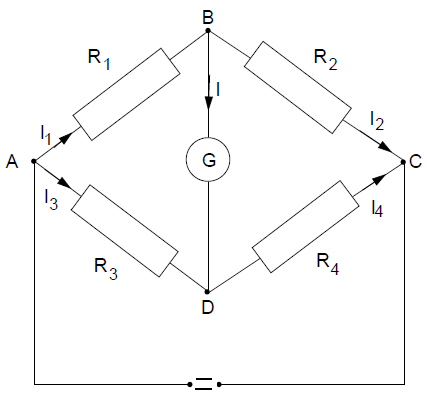
\includegraphics[scale=0.4]{Obecné zapojení stejnosměrného můstku}
    \captionsetup{justification=centering, font=footnotesize}
    \captionof{figure}{Obecné zapojení stejnosměrného můstku}
    \label{fig:Obecné zapojení stejnosměrného můstku}
    \vspace{30pt}
    \centering
    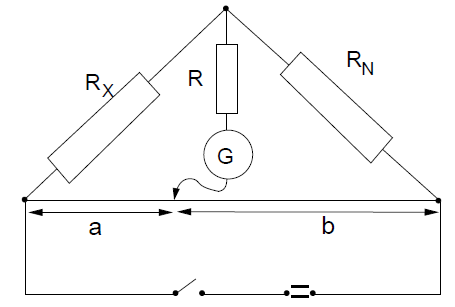
\includegraphics[scale=0.4]{Můstek s lineárním potenciometrem}
    \captionsetup{justification=centering, font=footnotesize}
    \captionof{figure}{Můstek s lineárním potenciometrem}
    \label{fig:Můstek s lineárním potenciometrem}
\end{minipage}
\newpage
\begin{minipage}[]{0.5\textwidth}
        Tímto můstkem budu měřit odpor dvou samostatných rezistorů. Poté změřím jejich odpor při sériovém a paralelním zapojení.
        \par Při sériovém zapojení se odpor $R_s$ vypočítá podle následujícího vzorce: 
        \begin{equation}
            R_s = R_1 + R_2
        \end{equation}
        Nejistotu vypočítáme podle následujícího vzorce: 
        \begin{equation}
            u(R_s) = \sqrt{u^2(R_1)+u^2(R_2)}
        \end{equation}

        \subsection{Rozložení potenciálu v okolí dvouvodičového vedení}
        Budu měřit rozložení elektrického potenciálu v blízkosti dvou vodičů v lázni s elektrolytem pomocí zařízení znázorněného na obrázku (\ref{fig:Střídavý můstek pro měření v elektrolytické vaně (a). Náhradní schéma elektrolytické vany (b)}).
            \par Netriviálním technickým řešením bylo připojení pohyblivého kontaktu, který je umístěn v rovině elektrolytové lázně a může se v ní volně pohybovat, ke grafickému tabletu, který bude snímat polohy pohyblivého kontaktu v rovině x y. 
            \par Každý bod na přímce příslušného potenciálu lze popsat veličinami $r_1$ a $r_2$. 
            \par Poloměrem $r_1$ a $r_2$ je parametr $\lambda$, který lze získat z následujícího vzorce: 
            \begin{equation}
                \lambda = e^{(\frac{2U}{\Delta U} -1)ln(\frac{h+a}{R})}
            \end{equation}
            kde $U$ je potenciál hladiny, $\Delta U$ je rozdíl napětí mezi vodiči, $a$ je vzdálenost mezi středem vodiče a bodem měření potenciálu, $h$ je vzdálenost mezi středy vodičů, $R$ je poloměr vodičů (vodiče jsou válce).
            \par Pro Apollonovy kružnice dále určím jejich y-novou souřadnici středu:
            \begin{equation}
                y_s = a \frac{\lambda^2 + 1}{\lambda^2 - 1}
            \end{equation}
            \begin{equation}
                a = \sqrt{h^2 - R^2}
            \end{equation}
            A jejich poloměr:
            \begin{equation}
                r_s = \sqrt{y_s^2 - a^2}
            \end{equation}
            \centering
            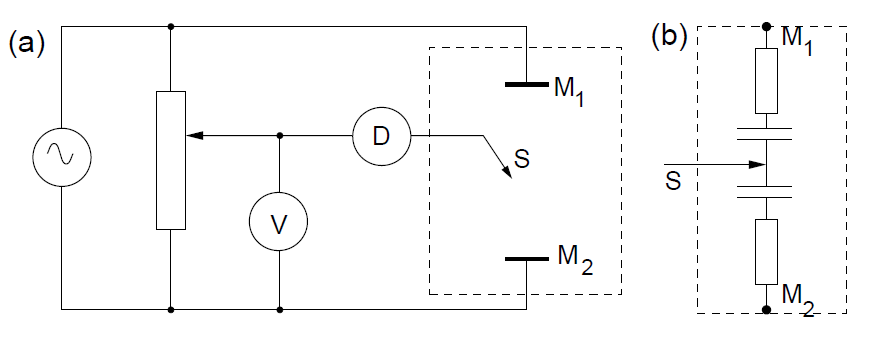
\includegraphics[scale=0.35]{Střídavý můstek pro měření v elektrolytické vaně (a). Náhradní schéma elektrolytické vany (b)}
            \captionsetup{justification=centering, font=footnotesize}
            \captionof{figure}{Střídavý můstek pro měření v elektrolytické vaně (a). Náhradní schéma elektrolytické vany (b)}
            \label{fig:Střídavý můstek pro měření v elektrolytické vaně (a). Náhradní schéma elektrolytické vany (b)}
            \vspace{10pt}
    \end{minipage}
    \hspace{10pt}
    \begin{minipage}[]{0.5\textwidth}
        \centering
            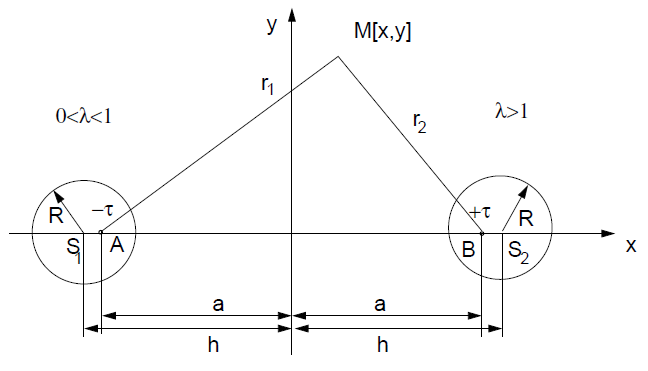
\includegraphics[scale=0.35]{Výpočet potenciálu v bodě M od dvou válcových nekonečných vodičů s poloměrem R, mezi nimiž je rozdíl potenciálů U}
            \captionsetup{justification=centering, font=footnotesize}
            \captionof{figure}{Výpočet potenciálu v bodě M od dvou válcových nekonečných vodičů s poloměrem R, mezi nimiž je rozdíl potenciálů U}
            \label{fig:Výpočet potenciálu v bodě M od dvou válcových nekonečných vodičů s poloměrem R, mezi nimiž je rozdíl potenciálů U}
        \vspace{20pt}
        \raggedright
        Při paralelním zapojení se odpor $R_p$ vypočítá podle následujícího vzorce: 
        \begin{equation}
            R_p = \frac{R_1 R_2}{R_1 + R_2}
        \end{equation}
        Nejistotu vypočítáme podle následujícího vzorce: 
        \begin{equation}
            u(R_p) = \frac{1}{(R_1 + R_2)^2} \sqrt{R_1^4u^2(R_1)+R_2^4u^2(R_2)}
        \end{equation}
        Při statistickém zpracování dat budu za hodnotu považovat aritmetický průměr a za nejistotu nejistotu aritmetického průměru.
        
        \section{Měření}
        \subsection{Měření odporu můstkovou metodou}
            Po zapojení rezistoru podle obvodu znázorněného na obrázku (\ref{fig:Můstek s lineárním potenciometrem}) jsem změnou hodnoty $a$ a změnou hodnot $R_N$ získal hodnoty $R_1$ a $R_2$ podle vzorce (2). 
            \begin{center}
                Hodnota $l$ = 100.0(1) [$cm$]
            \end{center}
            \centering
            \begin{tabular}{|c|c|c|c|c|c|c|}
                \hline
                a [$cm$] & $R_{N_1}$ [$\Omega$] & $R_1$ [$\Omega$] & $R_{N_2}$ [$\Omega$] & $R_2$ [$\Omega$] \\
                \hline
                30 & 240.0 & 102.9(5) & 1580.0 & 677(3)\\
                \hline
                50 & 90.1 & 90.1(4) & 680.0 & 680(3)\\
                \hline
                70 & 43.0 & 100.3(6) & 294.0 & 686(4)\\
                \hline
            \end{tabular}
            \captionsetup{justification=centering, font=footnotesize}
            \captionof{table}{Odpory pro jednotlivé rezistory}
            \vspace{10pt}
            \raggedright
            \par Z tabulki (1) vyplývá, že hodnoty odporu rezistorů $R_1$ a $R_2$ se rovnají:
            \begin{center}
                $R_1$ = 98(6) [$\Omega$]
                \par $R_2$ = 681(4) [$\Omega$]
            \end{center}
            \par Ze vzorců (3) a (5) vyplývá, že teoretické hodnoty odporů $R_{T_s}$ a $R_{T_p}$ se rovnají: 
            \begin{center}
                $R_{T_s}$ = 779(7) [$\Omega$]
                \par $R_{T_p}$ = 85(4) [$\Omega$]
            \end{center}
    \end{minipage}
\newpage
    \begin{minipage}[t]{0.5\textwidth}
    \vspace{-138pt}
        \begin{tabular}{|c|c|c|c|c|c|c|}
                    \hline
                    a [$cm$] & $R_{N_s}$ [$\Omega$] & $R_s$ [$\Omega$] & $R_{N_p}$ [$\Omega$] & $R_p$ [$\Omega$] \\
                    \hline
                    30 & 1473.0 & 631(3) & 260.0 & 111(6)\\
                    \hline
                    50 & 573.0 & 573(3) & 88.2 & 88.2(4)\\
                    \hline
                    70 & 187.0 & 436(3) & 34.4 & 87.3(5)\\
                    \hline
                \end{tabular}
                \captionsetup{justification=centering, font=footnotesize}
                \captionof{table}{Odpory rezistorů v sériovém a paralelním zapojení}
                \vspace{10pt}
                \raggedright
                \par Z tabulki (2) vyplývá, že hodnoty odporu rezistorů $R_s$ a $R_p$ se rovnají:
                \begin{center}
                    $R_s$ = ($550 \pm 80$) [$\Omega$]
                    \par $R_p$ = ($96 \pm 10$) [$\Omega$]
                \end{center}
        \subsection{Rozložení potenciálu v okolí dvouvodičového vedení} 
            Změnou hodnot $U$ získám polohy ekvipotenciálních čar pro různé hodnoty směru. Poté získám teoretické hodnoty poloh ekvipotenciálních čar. 
            \par Z měření se získají hodnoty poloměrů elektrod $R$ a vzdálenosti mezi nimi $h$:
            \begin{center}
                $R$ = 1.5 [$cm$]
                \par $h$ = 15 [$cm$]
                \par $a$ = 14.9 [$cm$]
                \par $\Delta U$ = 2 [$V$]
            \end{center}
            \raggedright
            \par Pro výpočty Apollónových kružnic použiji vzorce (7), (8), (9), (10).
            \vspace{20pt}
            \par \centering
            \begin{tabular}{|c|c|c|c|}
                    \hline
                    U [$V$] & $\lambda$ & $y_s$ [$cm$] & $r_s$ [$cm$] \\
                    \hline
                    0.25 & 0.11 & -15.3 & 3.2 \\
                    \hline
                    0.5 & 0.22 & -16.5 & 7.0 \\
                    \hline
                    0.75 & 0.47 & -23.5 & 18.2 \\
                    \hline
                    1 & 1 & - & - \\
                    \hline
                    1.25 & 2.11 & 23.5 & 18.2 \\
                    \hline
                    1.5 & 4.47 & 16.5 & 7.0 \\
                    \hline
                    1.75 & 9.44 & 15.3 & 3.2\\
                    \hline
                \end{tabular}
                \captionsetup{justification=centering, font=footnotesize}
                \captionof{table}{Teoretické výpočty rozložení ekvipotenciálních čar}
                \vspace{20pt}
                \raggedright
                Dále do grafu zakreslím všechny ekvipotenciální body odpovídající jednotlivým napětím $U$.
                \par Ekvipotenciály získané z hodnot $y_s$ a $r_s$ vyneseme do grafu.
                \par Získaný výsledek je vidět na obrázku (\ref{fig:Umístění ekvipotenciálů}).
    \end{minipage}
    \begin{minipage}[t]{0.5\textwidth}
        \centering
            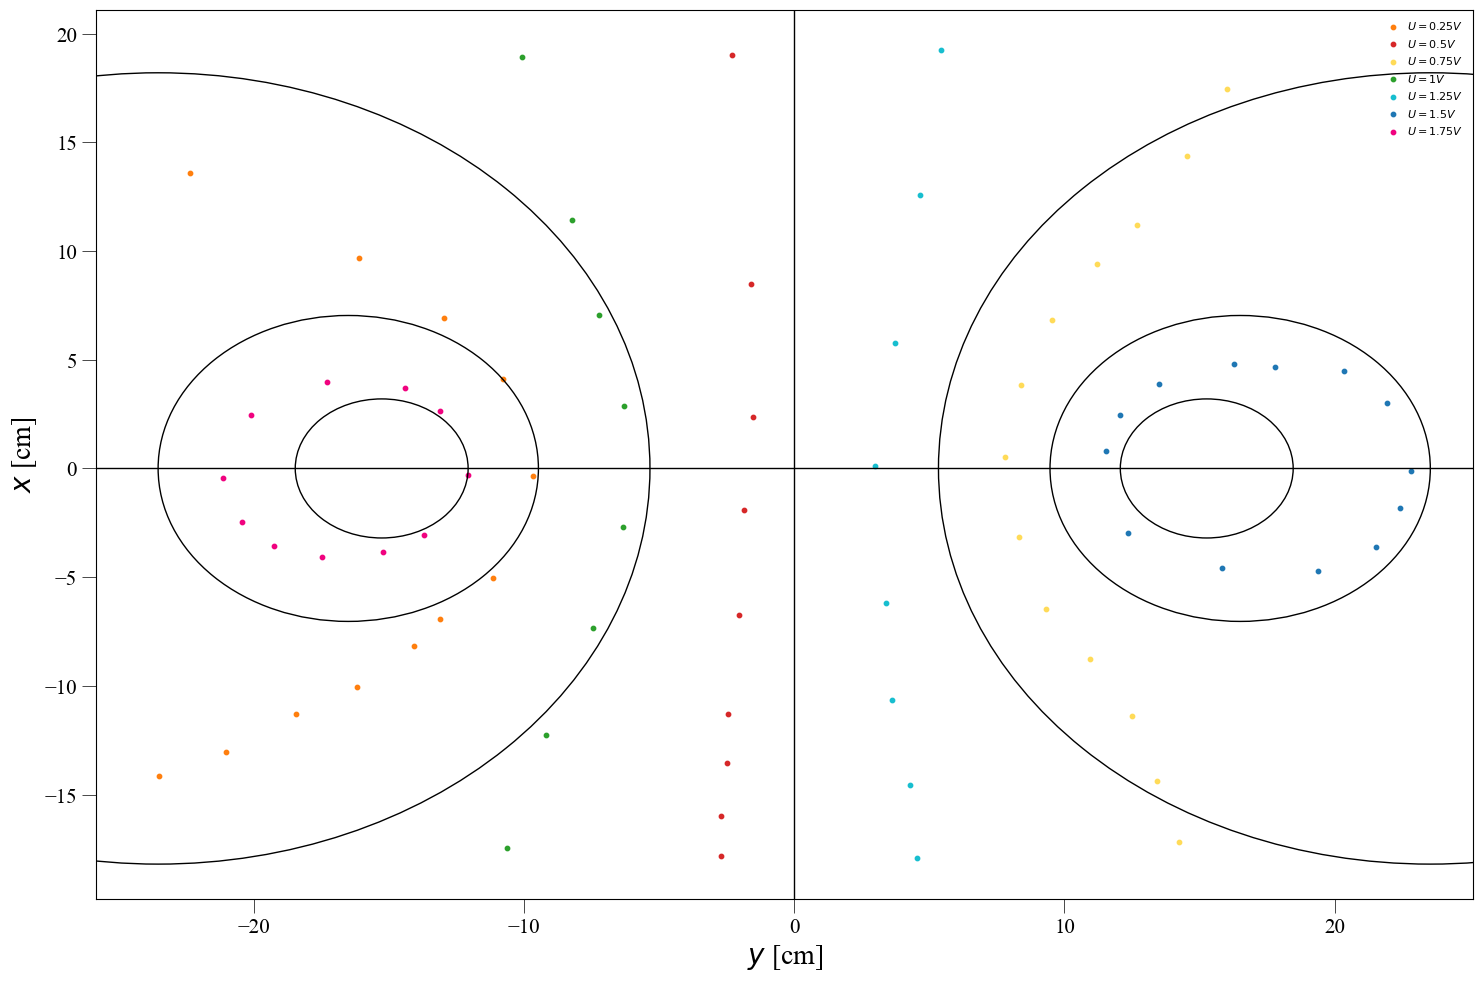
\includegraphics[scale=0.2]{equipotentials}
            \captionsetup{justification=centering, font=footnotesize}
            \captionof{figure}{Umístění ekvipotenciálů }
            \label{fig:Umístění ekvipotenciálů}
        \raggedright
        \section{Závěr}
        \subsection{Měření odporu můstkovou metodou}
        Získané hodnoty odporu jednotlivých rezistorů $R_1$ = 98(6) [$\Omega$] a $R_2$ = 681(4) $[\Omega]$  poměrně dobře odpovídají nominálním hodnotám uvedeným na rezistorech $R_{1_nom}$ = 101 $[\Omega]$ a $R_{2_nom}$ = 670 $[\Omega]$.
        \par Na druhé straně se teoretické ($R_{T_s}$ = 779(7) [$\Omega$], $R_{T_p}$ = 85(4) [$\Omega$]) a experimentální ($R_s$ = ($550 \pm 80$) [$\Omega$], $R_p$ = ($96 \pm 10$) [$\Omega$]) hodnoty odporů rezistorů v sériovém a paralelním zapojení od sebe výrazně liší (v rozmezí 1 $\sigma$). To může být způsobeno nepřesností měření. Například když byl $R_N$ zvolen v závislosti na $a$, lze jej přesněji nastavit zvýšením přesnosti měření galvanometrem $G$.
    \subsection{Rozložení potenciálu v okolí dvouvodičového vedení} 
        Jak je patrné z obrázku (\ref{fig:Umístění ekvipotenciálů}), teoretické a experimentální hodnoty ekvipotenciálů se neshodují. Zvláště výrazně se liší blíže ke středu mezi elektrodami. To může být způsobeno nepřesností měření vlnových minim na osciloskopu a také možným posunem polohy elektrod během měření. 
    \end{minipage}
\end{document}